%!TEX root = ../../../report.tex

\section{Geometrical dimensions of the frame} % (fold)
\label{sec:dimensions}

The selection of the final dimensions of RuBi corresponds to an iterative process in which power requirements have been the first constraint when assessing the size of the robot.
A first approach was taken from \cite{grimmer}, Manuscript I, where normalized values of power required per joint and per kilogram of the structure can be found.
The first iteration targeted a robot of dimensions $m = 1Kg$ and length from the hip joint to the tip toes of $L = 0.6 m$ for a fully stretched leg.
The final parameters from the last iteration can be found in ***%***chapter Results

Once estimated an overall length of the structure, the dimensions of each link were decided to be obtained based on the German section of the ISO 7250-2 \cite{iso_measurements} and the DIN 33402-2 \cite{din_measurements1} norms, following the idea of mimicking human-like motion as closely as possible.
These two norms are standard references in industry and were considered a general enough source of information.
Figure \ref{fig:human_measurements} depicts some of the human dimensions extracted from the norms and applied to the design of RuBi.
Their names and values for male between 18-65 year old and in percentile 50 can be found in table \ref{tab:din_proportions}.

\begin{figure}[h]
	\centering
	\begin{subfigure}[b]{0.3\textwidth}
        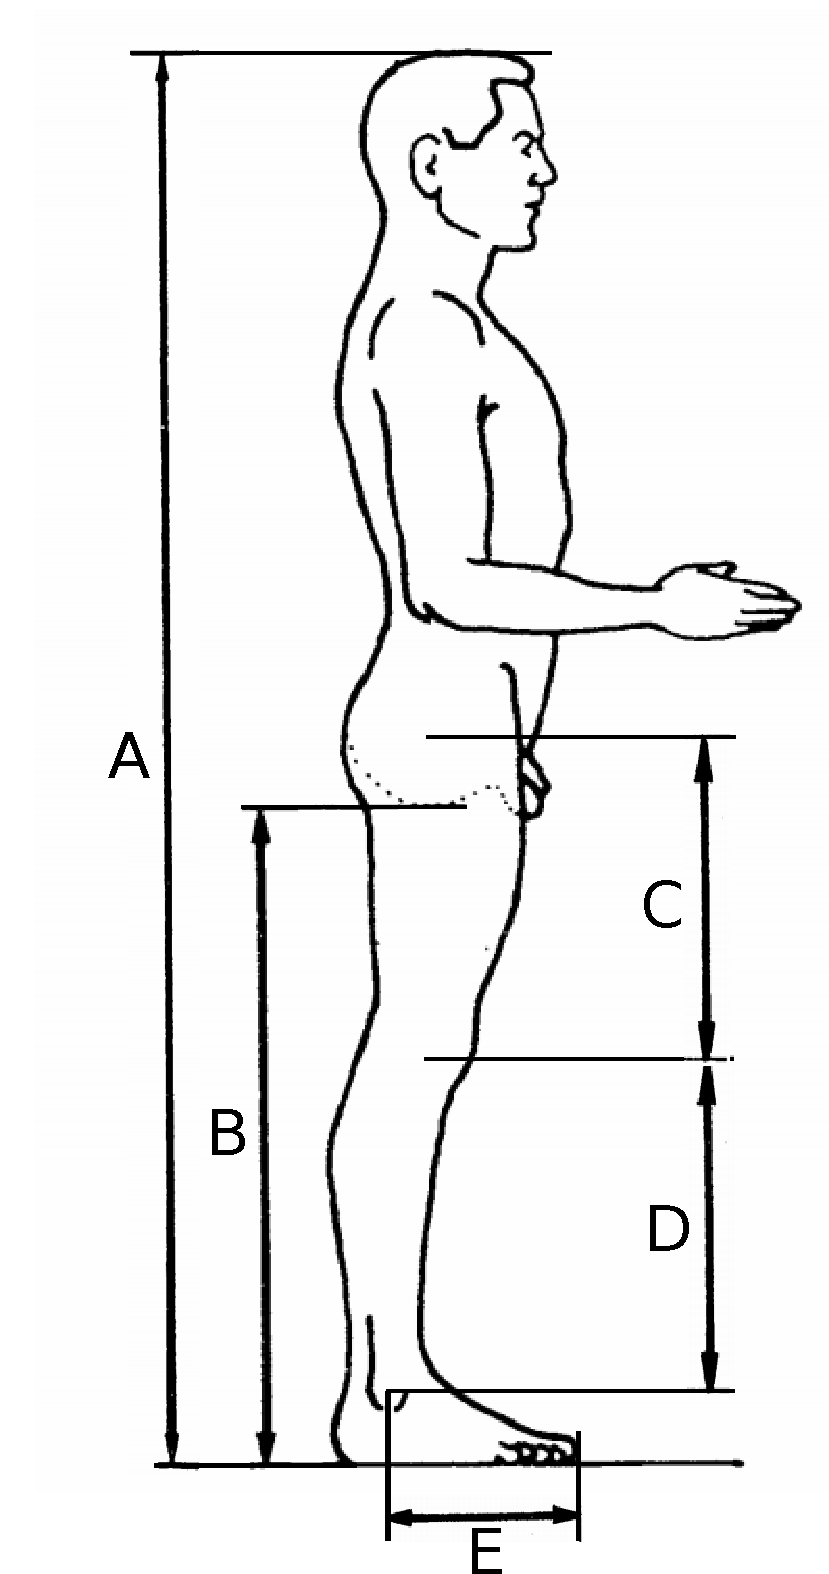
\includegraphics[width=\textwidth]{figures/din_measurements.pdf}
        \caption{Left foot}
        \label{fig:din1}
    \end{subfigure}
    \begin{subfigure}[b]{0.4\textwidth}
        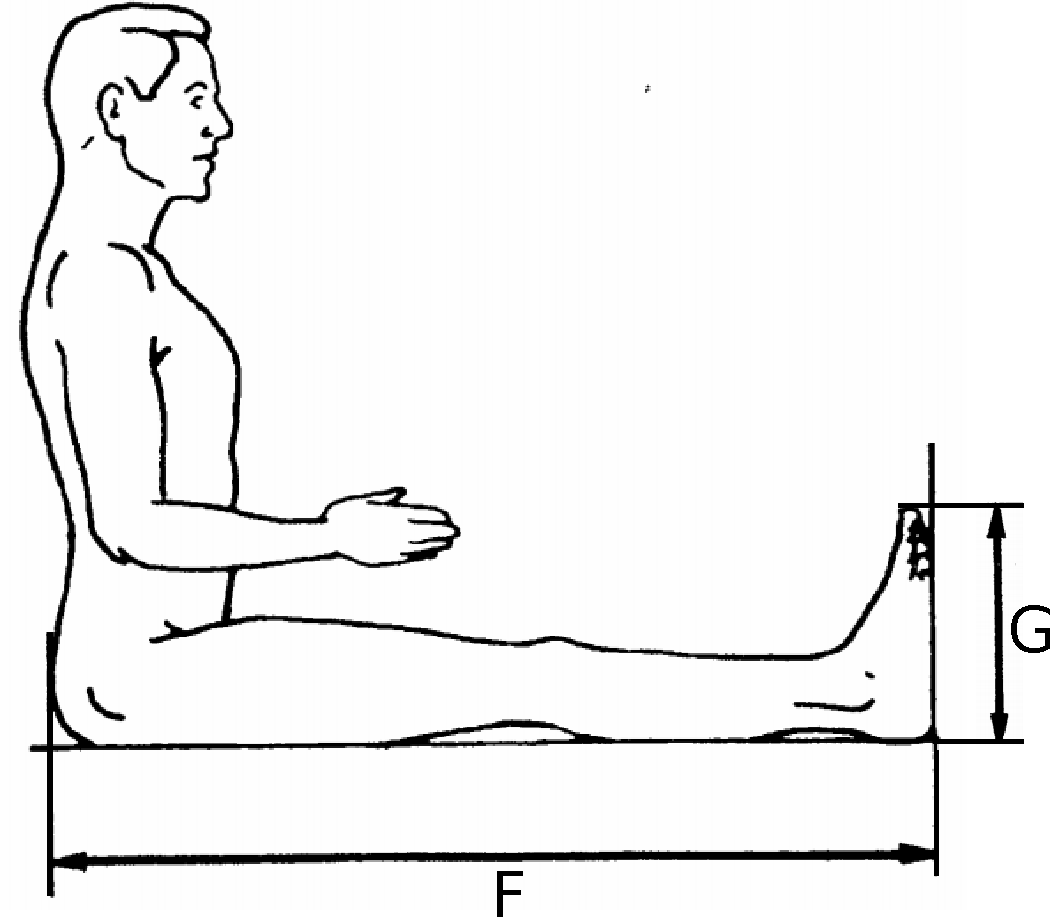
\includegraphics[width=\textwidth]{figures/din_measurements2.pdf}
        \caption{Hip}
        \label{fig:din2}
    \end{subfigure}
	\caption{Lower body measurements used for RuBi. Picture adapted from \cite{din_measurements1}.}
	\label{fig:human_measurements}
\end{figure}


\begin{table}
\begin{center}
	\begin{tabular}{c | c | c | c}
	  Index & Definition & Value & \% of Stature \\
	  \hline
	  A & Stature (body height) & ** & 100 \\
	  B & Crotch height & ** & ** \\
	  C & Femur height & ** & ** \\
	  D & Tibial height & Not in norm & **\\
	  E & Ankle-toe tip distance & Not in norm & ** \\
	  F & Buttocks-leg length & ** & ** \\
	  G & Sole length & ** & **
	\end{tabular}
	\caption{Human proportions from DIN 33402-2}
	\label{tab:din_proportions}
\end{center}
\end{table}

The dimensions needed to create a simplified model of one leg are the limbs lengths, which are the straight line distances measured from two consecutive joints.
They have been called $L_{i}$ where $i$ is the robot link + joint as per table \ref{tab:limb_index} and can be seen in Figure \ref{fig:kinematics}.
However, the norm does not determine all of them.

\begin{table}
\begin{center}
	\begin{tabular}{c | c | c}
	  $L_{i}$ & Limb \\
	  \hline
	  $L_{1}$ & Hip + thigh & C \\
	  $L_{2}$ & Knee + Foreleg & D\\
	  $L_{3}$ & Ankle + foot & E 
	\end{tabular}
	\caption{Limbs index}
	\label{tab:limb_index}
\end{center}
\end{table}

Since $C$ and $E$ are not standard measurements in industry, they have been obtained as follows:

\paragraph{The Femur height}
The crotch height, denoted as $B$ in the figure, has been averaged with the buttocks-leg length and the tibial height + an empirical approximation of the height of the ankle have been subtracted from the result, obtaining $C$.

\paragraph{The ankle-toe tip distance}
Since this distance is not standard either, it has been obtained once again adjusting the sole length with empirical measurements.

%% Here we just describe the process followed to obtain the final dimensions. 
%% The final results are shown in Chapter Results --> add tables and Froude number calculus


% section dimensions (end)